\chapter{آزمایش‌ها و نتایج}

\section{دادگان}

\subsection{مجموعه داده \lr{Cityscapes}}

مجموعه داده‌های \verb*|Cityscapes| یکی از پرکاربردترین مجموعه‌های داده برای مسائل تقسیم‌بندی معنایی است، که بر روی درک مفهومی صحنه‌های خیابانی شهری تمرکز دارد. این مجموعه شامل ۵۰۰۰ تصویر با برچسب‌گذاری دقیق و ۲۰۰۰۰ تصویر با برچسب‌گذاری خشن است، که برای ۳۰ کلاس معنایی مختلف آموزش دیده‌اند. تصاویر زیر مقایسه‌ای بین دو نوع برچسب‌گذاری ارائه می‌دهند.

\begin{figure}[ht]
	\centering
	\begin{subfigure}{0.45\textwidth}
		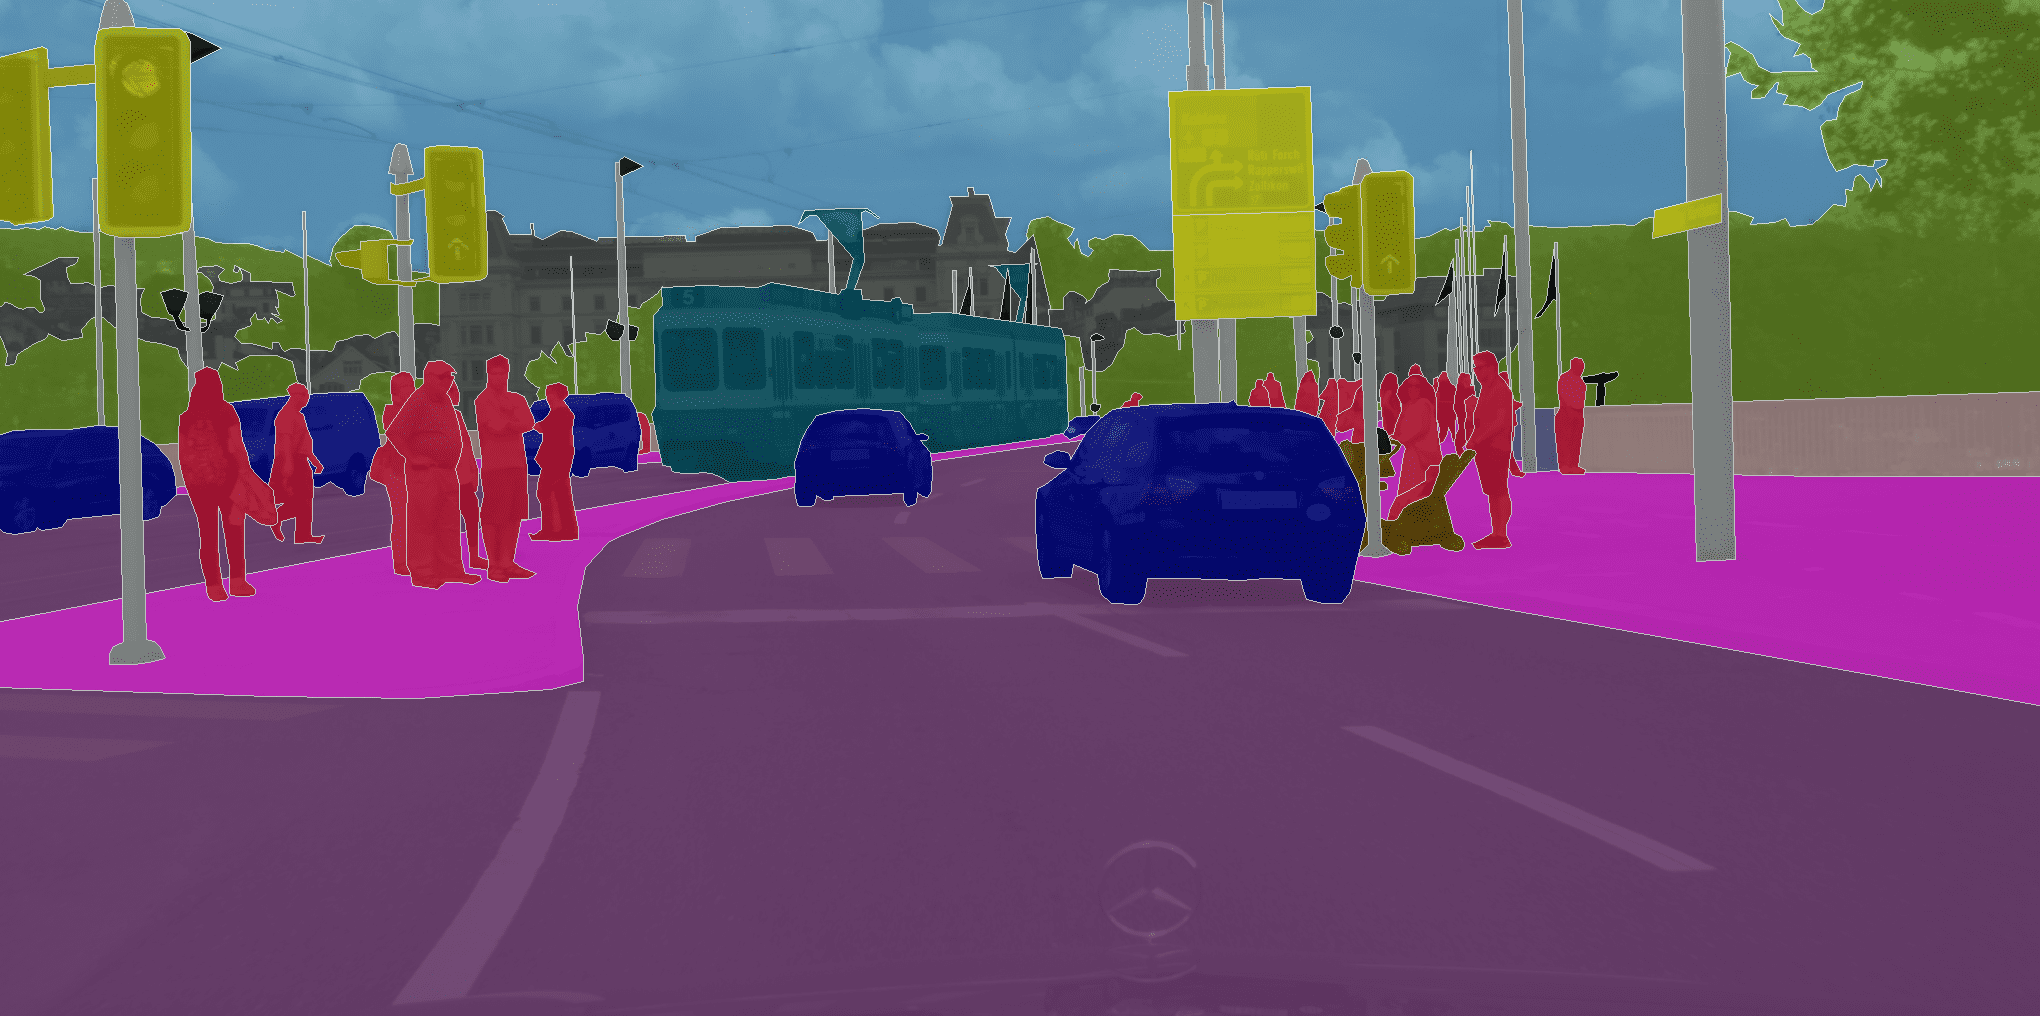
\includegraphics[width=\linewidth, height=0.2\textheight]{Images/Chapter2/Cityscapes/zuerich00.png}
		\caption{برچسب‌گذاری دقیق}
		\label{f64}
	\end{subfigure}\hfil
	\begin{subfigure}{0.45\textwidth}
		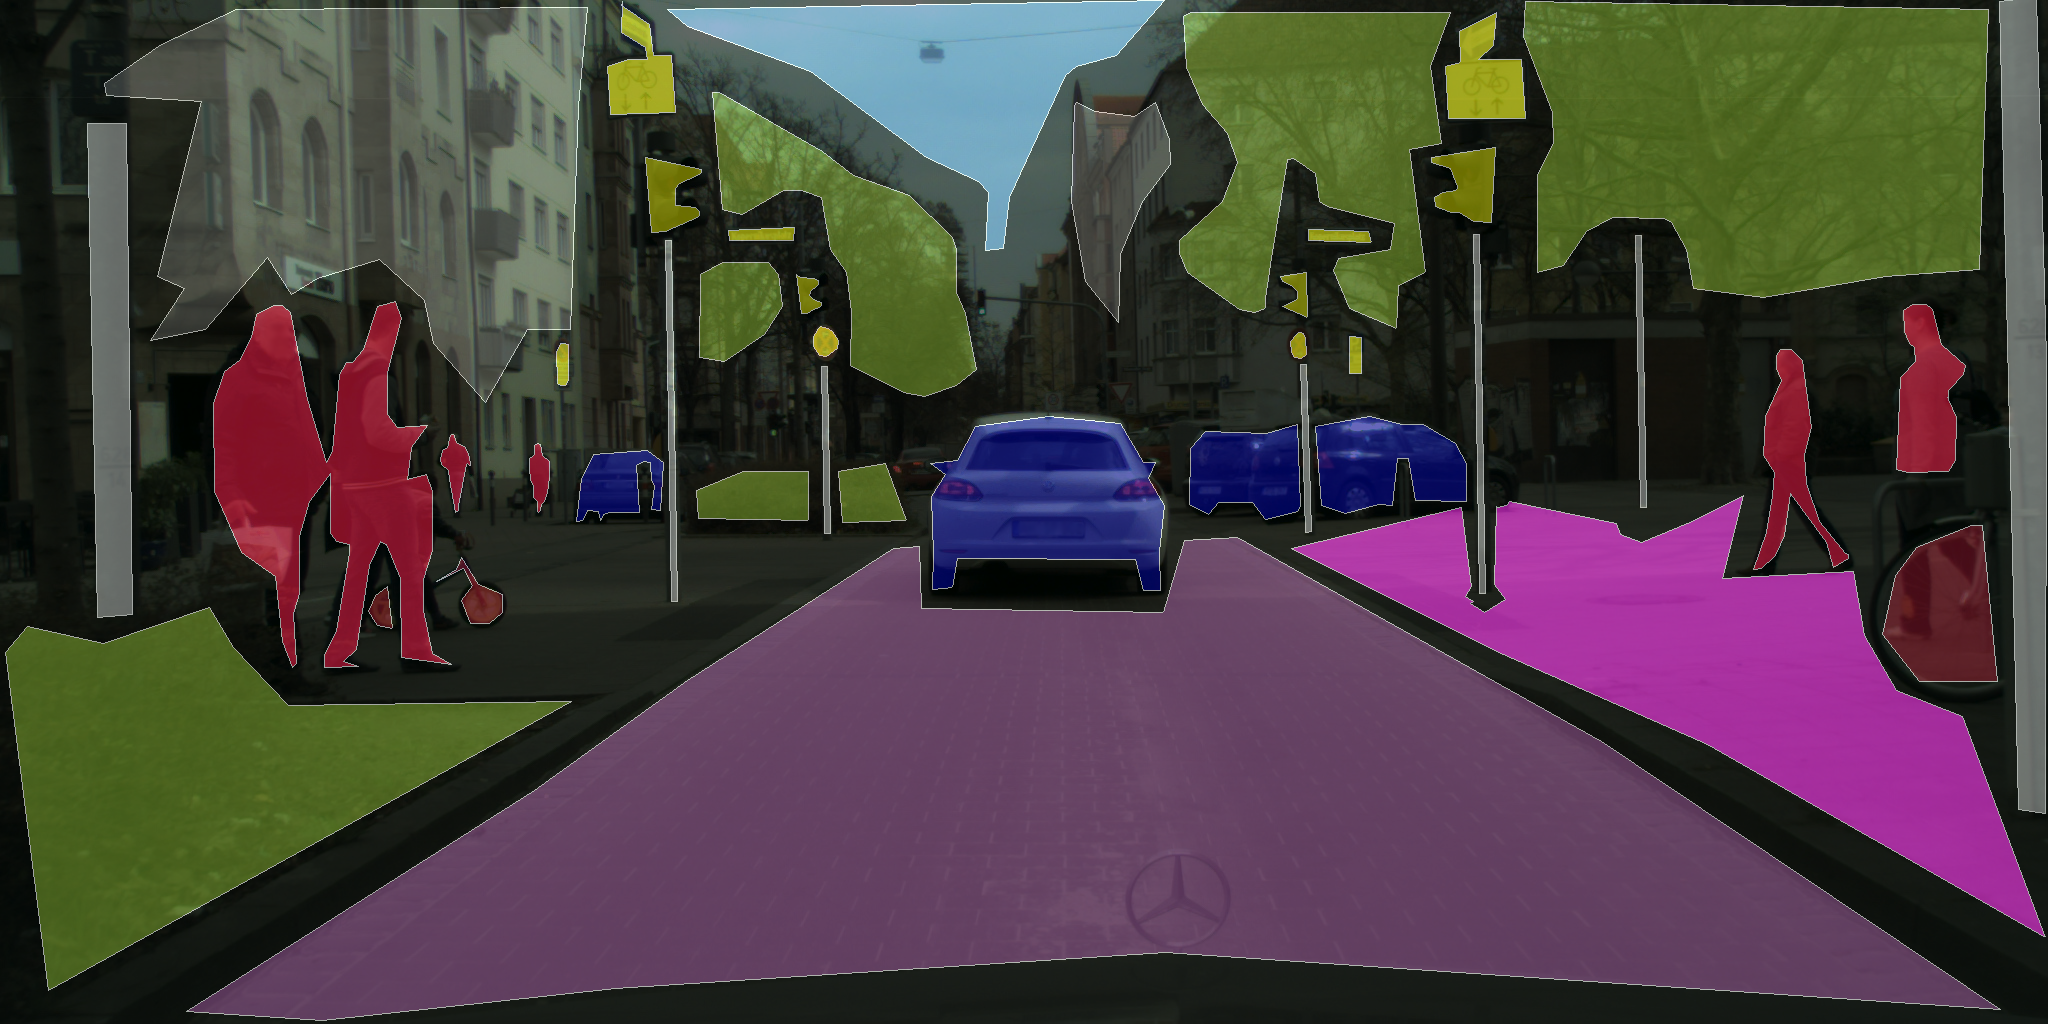
\includegraphics[width=\linewidth, height=0.2\textheight]{Images/Chapter2/Cityscapes/nuremberg00.png}
		\caption{برچسب‌گذاری خشن}
		\label{f65}
	\end{subfigure}
	\caption{انواع بر‌چسب‌گذاری دادگان \lr{Cityscapes}}
	\label{fig:fig1}
\end{figure}

ما در این پژوهش از ۵۰۰۰ تصویر با برچسب‌گذاری شده به شیوه دقیق استفاده خواهیم کرد، چراکه مراجع مورد استفاده قرار گرفته نیز از این نوع برچسب‌گذاری برای مقایسه استفاده کرده اند.

\subsection{مجموعه داده \lr{CamVid}}

در سال ۲۰۰۷، پایگاه داده ویدیویی با برچسب‌گذاری شهری کمبریج (\verb*|CamVid|)، از اولین مجموعه‌های داده تقسیم‌بندی معنایی برای خودروهای خودران، منتشر شد که در آن، ۷۰۰ تصویر از یک دنباله ویدیویی با مدت زمان ۱۰ دقیقه برچسب‌گذاری شد. برای گرفتن ویدیو، دوربین در جلوی ماشین قرار گرفته که دیدگاه مشابهی با راننده دارد. در این مجموعه داده ۳۲ دسته بندی معنایی وجود دارد.

\section{معیار‌های ارزیابی}

\subsubsection{زمان استنتاج}

برای اندازه‌گیری زمان استنتاج از معیار
\verb*|fps|
\LTRfootnote{Frame per second}
استفاده می‌کنیم تا سرعت زمان استنتاج مدل‌ها را با یکدیگر بررسی کنیم. به طبع هر چه
\verb*|fps|
بالاتری داشته باشیم برای ما مطلوب‌تر خواهد بود.


\subsubsection{بهره‌وری منابع}

در این معیار به سه مشخصه زیر می‌پردازیم تا دید بهتری به مقیاس هر مدل پیدا کنیم:

\begin{itemize}
	\item تعداد پارامتر ها: هر چه تعداد نورون‌های بیشتری داشته باشیم مدل سنگین تر می‌شود. تلاش بر آن است که مدل پیشنهادی سبک‌وزن (\lr{lightweight}) باشد.
	\item میزان مصرف مموری: متناسب با پیچیدگی مدل در تعداد و نوع عملیات‌ها میزان مصرف مموری در حین اجرا متغیر است.
	\item میزان مصرف حافظه: این مقدار با تعداد پارامتر‌ها نسبت مستقیم دارد، اما دید شهودی به مقیاس هر مدل می‌دهد.
\end{itemize}

\subsubsection{میانگین اشتراک بر اجتماع}

میانگین اشتراک بر اجتماع
\LTRfootnote{Mean intersection-over-union (Mean IoU)}
یک معیار پرکاربرد در مسائل بینایی ماشین
\LTRfootnote{Computer vision}
است که برای ارزیابی عملکرد مدل‌ها مورد استفاده قرار می‌گیرد و به وسیله محاسبه میزان تطابق بین ماسک تشخیص
\LTRfootnote{Prediction mask}
شیء پیش‌بینی شده توسط مدل و ماسک واقعی در تصویر عمل می‌کند. برای محاسبه این معیار، ابتدا
\verb*|IoU|
یا اشتراک بر اجتماع برای هر شیء در تصویر محاسبه می‌شود، سپس از آن‌ها میانگین گرفته می‌شود تا عملکرد کلی مدل در تشخیص شیء مورد ارزیابی قرار گیرد.

در اینجا اشتراک بر اجتماع هر دسته و میانگین کلی به صورت جدا سنجیده و مقایسه می‌شود.

\section{شرایط آزمایش}

برای ایجاد یک مقایسه عادلانه، دادگان مورد استفاده قرار گرفته را به دو بخش مجموعه‌داده آموزشی
\LTRfootnote{Training set}
و مجموعه‌داده صحبت‌سنجی
\LTRfootnote{Validation set}
تقسیم کردیم. تقسیم‌بندی به همانگونه که در دادگان اولیه انجام‌شده بود نگه‌داشته شد تا در مقایسه با مقاله‌های معتبر دچار مشکل نشویم.
تمامی مدل‌های پیاده سازی شده در چهارچوب پیاده‌سازی پایتورچ
\LTRfootnote{PyTorch framework}
پیاده‌سازی شده اند و تمامی آن‌ها بر روی سخت‌افزای با پردازنده
\verb*|AMD|
\verb*|Ryzen7|
\verb*|3.20|
\verb*|GHz|
و کارت گرافیکی
\verb*|NVIDIA|
\verb*|GeForce|
\verb*|GTX|
\verb*|3060|
\verb*|6GB|
انجام شده است.
\section{نتایج آزمایش و مقایسه}

در ابتدا به بررسی سرعت پردازش (
\verb*|fps|
) پرداخته می‌شود. در آزمایش فرض شده ۱۰ دسته‌بندی اشیاء داشته و تمامی تصاویر دارای ۳ کانال رنگی هستند. به دلیل محدودیت سخت‌افزاری روی پردازنده گرافیکی این مقایسه بر روی تصاویر با ابعاد ۲۰۴۸ در ۱۰۲۴ انجام نشده است. نتایج در جدول زیر قابل مشاهده است.

\begin{table}[ht]
	\centering
	\renewcommand{\arraystretch}{1.5}
	\begin{tabular}{|c|c|c|c|c|}
		\hline
		& $64$ \lr{x} $128$ & $128$ \lr{x} $256$ & $256$ \lr{x} $512$ & $512$ \lr{x} $1024$ \\ \hline
		\lr{UNet} 		& $99.11$ & $95.47$ & $42.8$ & $7.42$ \\ \hline
		\lr{SQNet}  	& $94.01$ & $96.06$ & $41.86$ & $19.66$ \\ \hline
		\lr{ENet}  		& $70.55$ & $64.81$ & $34.98$ & $3.46$ \\ \hline
		\lr{FastSCNN}  	& $46.63$ & $46.55$ & $47.00$ & $33.63$ \\ \hline
		\lr{SegNet} 	& $18.84$ & $17.65$ & $14.99$ & $12.92$ \\ \hline
	\end{tabular}
	\caption{مقایسه شاخص \lr{fps}}
	\label{Table1}
\end{table}

علت گرفتن نتایج ضعیف‌تر نسبت به مقاله‌های اصلی، ضعیف‌تر بودن کارت گرافیکی استفاده شده و تفاوت‌های احتمالی در پیاده‌سازی‌های صورت گرفته است.



\section{خلاصه}